\documentclass[11pt,a4paper]{article}
\usepackage[utf8x]{inputenc}
\usepackage{graphicx}
\usepackage{esdiff}
\usepackage[english]{babel}
\usepackage{color}
\usepackage{booktabs}
\usepackage{tabularx}	
\usepackage{float}
\usepackage{enumitem}
\usepackage{epstopdf}
\usepackage{afterpage}
\usepackage{caption}
\usepackage{subcaption}
\captionsetup[table]{oneside , margin = {2cm, 0cm},
	justification=RaggedRight, singlelinecheck = false }
\usepackage{subcaption}
\usepackage{mathtools}
\usepackage{multicol}
\usepackage{algorithm2e}
\usepackage{microtype}
\usepackage{titling}
\usepackage{amsmath}
\usepackage{verbatim}
\usepackage{tasks}
\usepackage[colorlinks=true]{hyperref} % the option is there to remove the square around links which is what I don't like.
\usepackage{comment}
\usepackage{perpage} 
\MakePerPage{footnote} % Reset the footnote counter perpage. may require to run latex twice.
\usepackage{commath} % for absolute value
\usepackage[margin=2cm]{geometry} % This is here to fit more text into the page.

\setcounter{secnumdepth}{1}  % This removes the numbering from the subsections.
% If you want the numbering of the subsection level just remove this line
\usepackage{titling}
\newcommand{\subtitle}[1]{%
	\posttitle{%
		\par\end{center}
	\begin{center}\large#1\end{center}
	\vskip0.5em}%
}

\setlength{\parindent}{0pt} % No indentation for paragraphs. Because that is just old.
\setlength{\parskip}{\baselineskip} % Instead use vertical paragraph spacing.

\fontencoding{T1} % the better font encoding.
\title{\textsc{Lateral vibrations of a beam}}
\subtitle{\textsc{Mechanical vibrations}}	
%\date{11/06/2020}
\author{Giorgio Checola}

\makeatletter
\def\@maketitle{
\graphicspath{ {./images/} }
\begin{center}
	
\includegraphics[width=75mm]{images/Unitn.png} \\
	\vspace{10mm}
	\LARGE{UNIVERSIT\`A DEGLI STUDI DI TRENTO}
	\large
	
	Department of Industrial Engineering\\
	
	
	\vspace{15mm}
	\item { \Large Master's degree in \emph{Mechatronics Engineering}}
	\vspace{3mm}			
	\item { \Large Course of Mechanical vibrations} \\			
	\vspace{2mm}
	Laboratory experience\\
	
	\vspace{12mm}		
	
	\item {\Huge \@title } 

	\vspace{7mm}
	
	\begin{flushleft}
		\textbf{Professors:\hfill Students:} \\
		\smallskip
		Daniele Bortoluzzi \hfill Giorgio Checola\\
		Davide Vignotto
	\end{flushleft}
	
	\vfill
	Academic Year 2019 - 2020
	
\end{center}
}
\makeatother

\begin{document}

\graphicspath{ {./images/} }
\maketitle
\thispagestyle{empty}
\newpage
\thispagestyle{empty}
\mbox{}
\newpage


\section*{Introduction}	
This report concerns the laboratory experience of year 2019-2020. We studied the behaviour of a beam when it is excited by forces and observed the lateral vibrations that are generated during different tests. We used accelerometers, in different positions of the beam, to acquire data, which are the accelerations produced by the excitation.
The picture below shows the scheme of the analytical model of the system: as you can see, it is blocked from two pins at both ends.

\begin{figure}[H]
	\centering
	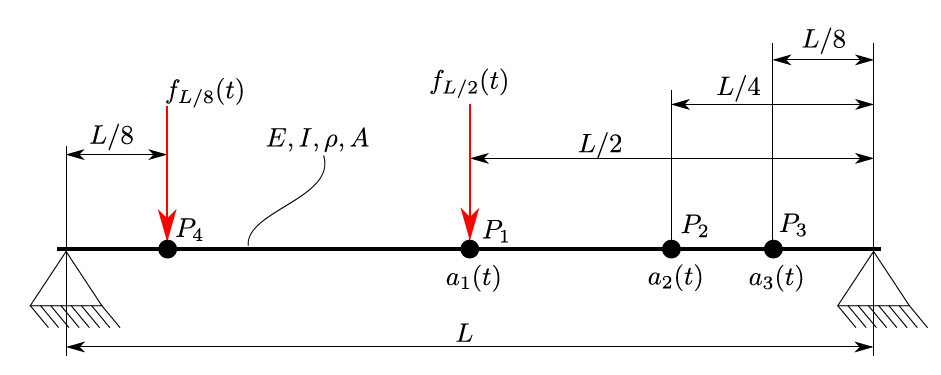
\includegraphics[width=150mm]{images/model.png}
	\caption{Model of the beam}
	\label{scheme}
\end{figure}

Before starting with the experimental part, it has been necessary to build the analytical model of the beam, for which we used these parameter values: 

\medskip

\begin{table}[h]
	\centering
	\begin{tabular}{c c c c} 
		\toprule
		\textbf{Name} & \textbf{Value} & \textbf{Unit} & \textbf{Description} \\ 
		\midrule	    		   	    		
		$E$     & 206  & $GPa$            & Young modulus \\	    		
		$\rho$  & 7850 & $\frac{kg}{m^3}$ & mass density \\	    		   
		$A$     & 111  & $mm^2$                 & area of the beam cross-section \\
		$I$     & 6370 & $mm^4$           & moment of inertia of the beam cross-section \\
		$L$     & 0.7  & $m$              &length of the beam\\
		$\xi_{1}$ & 0.05 & - &damping ratio of the first mode\\
		$\xi_{2,3,4}$ & 0.01 & - & damping ratio of the second, third and fourth mode\\
		\bottomrule
	\end{tabular}
	\caption{Parameters of the beam}
	\label{parameter}
\end{table}
\newpage

\section{Analytical model}
In this part of the project I preferred to use Maple since it is useful for analytic calculations and symbolic computation.

\begin{enumerate}
	\item As reference frame of the system I chose the left pin to be pratical. \\
	In order to find the values of the first five natural frequencies I followed the procedure explained in class.
	\begin{itemize}
		\item Starting from the definition of displacement $W(x)$ and momentum $M(x)$ (we exploit the separation of variable and consider the free vibration of a uniform beam):
		\begin{equation*}
			W(x)=c_1\cos(\beta x)+c_2\sin(\beta x)+c_3\cosh(\beta x)+c_4\sinh(\beta x)
		\end{equation*}
		\begin{equation*}
			M(x)=EI\frac{d^2 W}{dx^2}\,, \; \; \; \beta=\omega_n^2 {\frac{\rho A}{EI }}
		\end{equation*}
		
		\smallskip
		
		\item Writing the boundary conditions for a pinned-pinned beam:
		
		\smallskip
		
		\begin{tasks}(2)
			\task[$\rightarrow$] $W(0)=0$
			\task[$\rightarrow$] $W(L)=0$
			\task[$\rightarrow$] $M(0)=0$
			\task[$\rightarrow$] $M(L)=0$
		\end{tasks}	

		\smallskip
		
		In both joints there is no possibility to have a lateral displacement, moreover the beam is free to rotate, and so there is no external action that tends to keep the beam fixed.
		Finally we obtained:
		
		\begin{equation*}
			\left[\begin {array}{c} {c_1}+{c_3}=0 \\ 
			\noalign{\medskip}-EI{\beta}^{2} \left( {c_1}-{c_3} \right)=0 \\
			\noalign{\medskip}{c_1}\cos(\beta L)+{c_2}\sin(\beta L) +{c_3}\cosh(\beta L) +{c_4}\sinh(\beta L) =0\\
			\noalign{\medskip}-EI{\beta}^{2}({c_1}\cos(\beta L) +{c_2}\sin(\beta L)-{c_3}\cosh(\beta L)-{c_4}\sinh(\beta L))=0 \end {array} \right]		
		\end{equation*}	
		 
		 \smallskip
		 
		\item Solving the equations to get the constants and the values of $\beta$ which satisfy the equalities: I got c1 and c3 that are equal to 0 and substituted their values in the other two equations which I wrote in matrix form.
		\begin{equation*}
		\begin{bmatrix}
			\sin(\beta L)            & \sinh(\beta L) \\ \noalign{\medskip}
			-EI\beta^2 \sin(\beta L) & EI\beta^2 \sin(\beta L)
		\end{bmatrix} \begin{bmatrix} c_2 \\ c_4 \end{bmatrix} =
		\begin{bmatrix} 0 \\ 0 \end{bmatrix}	
		\end{equation*}
		I want non trivial solution, so I imposed the determinant of the 2x2 matrix equal to 0 and solved for $\beta$.
		\begin{equation}
		2{\beta}^{2}\sin(\beta L) EI\sinh(\beta L)=0		
		\end{equation}
		I took the first five values of the real solutions of $\beta$
		since I want only the first five natural frequencies. By knowing that $\omega_n=\beta^2 \sqrt{\frac{EI}{\rho A}}$ I found these values and relative frequencies:
		
		\begin{table}[h]
			\centering
			\begin{tabular}{c c c c c c} 
				\toprule
				\textbf{n°} & \textbf{1} & \textbf{2} & \textbf{3} & \textbf{2} & \textbf{2} \\
				\midrule	    		   	    		
				$\omega_n$ [$rad/s$] & 781.6470157 & $3126.588063$ & 7034.823141 & 12506.35225 & 19541.17539 \\
				\midrule	    		
				$f$ [$Hz$]  & 124.4029863 & 497.6119452 & 1119.626877 & 1990.447781 & 3110.074658 \\	    		   
				\bottomrule
			\end{tabular}
			\caption{Values of the first five natural frequencies and related frequencies}
		\end{table}
		
		
	\end{itemize}	
	For mode shapes I used the third boundary condition equation substituting one of the $\beta$ values (the solutions do not change). You can see that $c_4=0$, then I chose $c_2=1$ otherwise every constants would have been null. 
	Finally I obtained the first five mode shapes that I was searching for, shown in the figure below.
	
	\begin{figure}[H]
		\begin{subfigure}[b]{0.3\textwidth}
			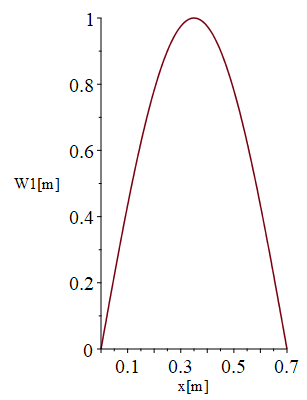
\includegraphics[width=55mm]{images/1_modeshape1.png}
			\caption{$W_1(x)$}
		\end{subfigure}
		\hfill
		\begin{subfigure}[b]{0.3\textwidth}
			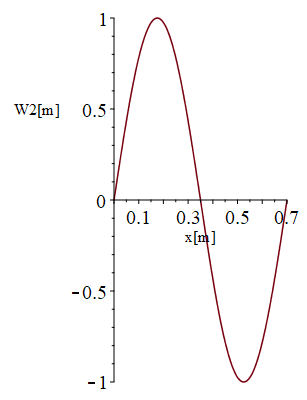
\includegraphics[width=55mm]{images/1_modeshape2.png}
			\caption{$W_2(x)$}
		\end{subfigure}
		\hfill
		\begin{subfigure}[b]{0.3\textwidth}
			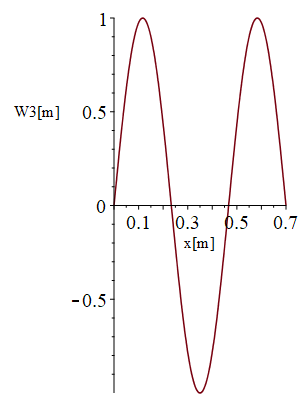
\includegraphics[width=55mm]{images/1_modeshape3.png}
			\caption{$W_3(x)$}
		\end{subfigure}
	\end{figure}

	\begin{figure}[H]
		\begin{subfigure}[b]{0.5\textwidth}
			\centering
			\includegraphics[width=55mm]{images/1_modeshape4.png}
			\caption{$W_4(x)$}
		\end{subfigure}
		\hfill
		\begin{subfigure}[b]{0.5\textwidth}
			\centering
			\includegraphics[width=55mm]{images/1_modeshape5.png}
			\caption{$W_5(x)$}
		\end{subfigure}
		\caption{First five mode shapes of the pinned-pinned beam}
	\end{figure}

	
	\medskip
	
	\item Using the mode superposition principle and exploiting the orthogonality of modal shapes, I built the analytical model of the pinned-pinned beam including also the damping factor.\\
	I need to approximate the motion of the system accordingly to Eq 1.
	
	\begin{equation}
	w(x,t)=\sum_{n=1}^{\infty} W_{n}(x) q_{n}(t) \approx \sum_{n=1}^{4} W_{n}(x) q_{n}(t)
	\end{equation}
	
	\newpage
	
	Let's consider the forced vibrations of the beam: I firstly computed the two external force f(x,t) in $P_1$ and $P_4$:
	\begin{enumerate}
		\item $f(x,t)=\delta(x-\frac{L}{2})h(t)$
		\item $f(x,t)=\delta(x-\frac{L}{8})h(t)$
	\end{enumerate}	
	where $\frac{L}{2}$ and $\frac{L}{8}$ are the distances of the points of application of the two forces from the left pin.
	
	\smallskip
	
	Then I found the related modal component $Q_m(t)$ truncated at the forth modal shapes and the modal mass $b_m$ using the formulas:
	\begin{align*}
	&Q_{m}=\int_{0}^{L} W_{m} f(x,t) dx\\
	&b_{m}= \int_{0}^{L}  W_{m}^2 dx
	\end{align*}
	Substituting everything in the modal coordinate equation, I solved it using Laplace Transform with zero initial conditions as a function of $q_n(s)$ (the exact values are shown in the Maple file).
	\begin{equation}
	\frac{d^2 dq_n}{dt^2} + 2\xi_n\omega_n\frac{dq_n}{dt} + \omega_n^2q_n = \frac{1}{\rho Ab}Q_n
	\end{equation}
	\begin{equation}
	s^2q_n(s)+2\xi_n\omega_n\cdot q_n(s)+\omega_n^2q_n(s) = \frac{1}{\rho Ab}Q_n
	\end{equation}
	The results for the force applied in P1:
	\begin{equation*}
	\left[ \begin {array}{c} {q_1}(s) 
	\\ \noalign{\medskip}{q_2}(s) \\ \noalign{\medskip}{q_3}(s) \\ \noalign{\medskip}{q4}(s)\end {array} \right] = \left[ \begin {array}{c} \frac{2h(s){L}^{3}} {2\xi_{{1}}\sqrt {{\frac {EI}{\rho A}}}{\pi}^{2}s\rho A{L}^{2}+{s}^{2}\rho A{L}^{4}+EI{\pi}^{4}}
	\\ \noalign{\medskip}0\\ \noalign{\medskip}\frac{-2h(s){L}^{3}}{ 18\xi_{{3}}\sqrt {{\frac {EI}{\rho A}}}{\pi}^{2}s\rho A{L}^{2}+{s}^{2}\rho A{L}^{4}+81EI{\pi}^{4}}
	\\ \noalign{\medskip}0\end {array} \right] 		
	\end{equation*}
	
	And for the force applied in P4
	\begin{equation*}
	\left[ \begin {array}{c} {q_1}(s) \\ \noalign{\medskip}{q_2}(s) \\ \noalign{\medskip}{q_3}(s) \\ \noalign{\medskip}{q_4}(s) \end {array} \right] = \left[ \begin {array}{c} \frac{2h(s)\sin(\frac {\pi}{8}){L}^{3}}{(2\xi_{{1}}\sqrt{{\frac {EI}{\rho A}}}{\pi}^{2}s\rho A{L}^{2}+{s}^{2}\rho A{L}^{4}+EI{\pi}^{4})}\\ \noalign{\medskip}\frac{h(s)\sqrt{2}{L}^{3}} {(8\xi_{{2}}\sqrt{{\frac{EI}{\rho A}}}{\pi}
		^{2}s\rho A{L}^{2}+{s}^{2}\rho A{L}^{4}+16\,EI{\pi}^{4})}\\ \noalign{\medskip}\frac{2h(s)\sin(\frac {3\pi}{8}){L}^{3}}{(18\xi_{{3}}\sqrt {{\frac {EI}{\rho A}}}{\pi}^{2}s\rho A{L}^{2}+{s}^{2}\rho A{L}^{4}+81EI{\pi}^{4})}\\ \noalign{\medskip}\frac{2h(s){L}^{3}}{(32\xi_{{4}}\sqrt {{\frac {EI}{\rho A}}}{\pi}^{2}s\rho A{L}^{2}+{s}^{2}\rho A{L}^{4}+256EI{\pi}^{4})}\end {array} \right] 		 	
	\end{equation*}
	
	Finally, once obtained $q_n(s)$, I got $w(x,s)$ as desired.
	
	\medskip
	
	\item In order to compute the analytical transfer function, I divided by $h(s)$ the beam displacement function $w(x,s)$; I substituted the position of the accelerometer, and multiplied by $s^2$ since I want the relation between an acceleration and a force, not between a position and a force. \\
	Since I have 3 accelerometers and 2 forces I got 6 transfer function $H_{ij}=\frac{A_i(s)}{F_j(s)}$. 
	
	\medskip
	
	\item The plot of the different transfer functions are visible in the following figures: $s$ has been replaced by $\iota\omega$ to get the frequency response functions; the frequency range is {$20\div2230$} Hz.
	
	\begin{figure}[H]
		\centering
		\begin{subfigure}[b]{0.3\textwidth}
			\centering
			\includegraphics[width=55mm]{images/1_tf1_1.png}
			\caption{$H_{11}(\iota\omega)$}
		\end{subfigure}
		\hfill
		\begin{subfigure}[b]{0.3\textwidth}
			\centering
			\includegraphics[width=55mm]{images/1_tf1_2.png}
			\caption{$H_{21}(\iota\omega)$}
		\end{subfigure}
		\hfill
		\begin{subfigure}[b]{0.3\textwidth}
			\centering
			\includegraphics[width=55mm]{images/1_tf1_3.png}
			\caption{$H_{31}(\iota\omega)$}
		\end{subfigure}
	\end{figure}

	\begin{figure}[H]
		\centering
		\begin{subfigure}[b]{0.3\textwidth}
			\centering
			\includegraphics[width=50mm]{images/1_tf2_1.png}
			\caption{$H_{14}(\iota\omega)$}
		\end{subfigure}
		\hfill
		\begin{subfigure}[b]{0.3\textwidth}
			\centering
			\includegraphics[width=55mm]{images/1_tf2_2.png}
			\caption{$H_{24}(\iota\omega)$}
		\end{subfigure}
		\hfill
		\begin{subfigure}[b]{0.3\textwidth}
			\centering
			\includegraphics[width=55mm]{images/1_tf2_3.png}
			\caption{$H_{34}(\iota\omega)$}
		\end{subfigure}
		\caption{Transfer function $H_{ij}(\iota\omega)$ between force and  acceleration, $i=P_1,P_2,P_3$ and $j=P_1,P_4$}
	\end{figure}

	Observing carefully, you can see that each plot includes two or more resonant peaks in proximity of the natural frequencies found previously, due to the fact that we computed the transfer function starting from the equation (4) and (2), and so the poles coincide with the natural frequencies of the free vibrations case. The minimal difference could be due to the dissipating term.\\ Moreover the position of the force and the accelerometers affect the graphs causing peak cancellation if their position coincide with a node.
	
	\medskip
	
	\item Now let's consider the fixed-fixed beam, with the same characteristics of before. \\
	I want to compute the analytical values of the natural frequencies and numerically evaluate those inside the frequency range of interest $f_{range}$. \\
	I followed the same procedure of question 1.
	The boundary conditions are different from before:
	
	\smallskip
	
	\begin{tasks}(2)
		\task[$\rightarrow$] $W(0)=0$
		\task[$\rightarrow$] $W(L)=0$
		\task[$\rightarrow$] $\frac{dW}{dx}(0)=0$
		\task[$\rightarrow$] $\frac{dW}{dx}(L)=0$
	\end{tasks}	
	
	\medskip
	
	In this case c1 and c2 are not 0, but they are function of c3 and c4; I substitute them in the other two equations; I tried to solve the determinant but there are no analytical valid solutions. Therefore I did it numerically with the function \texttt{fsolve} taking the first five values of $\beta$ and finally I computed natural frequencies and their corresponding Hz values, and see if they lie inside the range.
	
	\begin{table}[H]
		\centering
		\begin{tabular}{c c c c c c} 
			\toprule
			\textbf{n°} & \textbf{1} & \textbf{2} & \textbf{3} & \textbf{2} & \textbf{2} \\
			\midrule	    		   	    		
			$\omega_n$ [$rad/s$] & 1771.906055 & 4884.327263 & 9575.234362 & 15828.34881 & 23644.82237 \\
			\midrule	    		
			$f$ [$Hz$]  & 282.0076073 & 777.3648276 & 1523.945880 & 2519.159954 & 3763.190357 \\	    		   
			\bottomrule
		\end{tabular}
		\caption{Values of the first five natural frequencies and related frequencies}
	\end{table}

	You can see that only the first 3 are inside the range. Then I found the relationship between $c_3$ and $c_4$, chose $c_4=1$ as reference, and found the relative $c_3$ values.Finally I obtained the plots of mode shapes.
	
	\begin{figure}[H]
		\centering
		\begin{subfigure}[b]{0.3\textwidth}
			\centering
			\includegraphics[width=55mm]{images/1_5modeshape1.png}
			\caption{$W_1(x)$}
		\end{subfigure}
		\hfill
		\begin{subfigure}[b]{0.3\textwidth}
			\centering
			\includegraphics[width=55mm]{images/1_5modeshape2.png}
			\caption{$W_2(x)$}
		\end{subfigure}
		\hfill
		\begin{subfigure}[b]{0.3\textwidth}
			\centering
			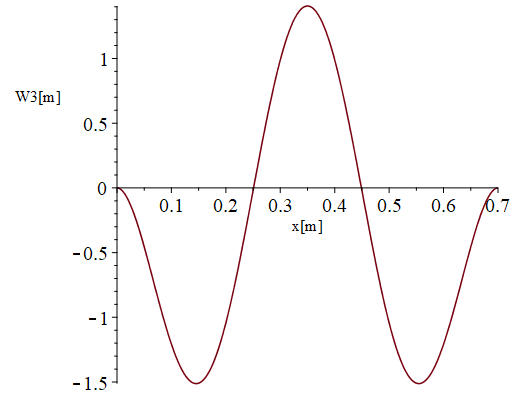
\includegraphics[width=55mm]{images/1_5modeshape3.png}
			\caption{$W_3(x)$}
		\end{subfigure}
		\caption{First three mode shapes of fixed-fixed beam}
	\end{figure}
	
	
\end{enumerate}			

\newpage

\section{Noise analysis}
Once concluded the analytical model of the system, I went on to the experiment. In this part the noise affecting the measurements was collected. There are no external force. \\
The data that we are interested in are: time($s$), force($N$), acceleration of accelerometer 1 ($m/s^2$), acceleration of accelerometer 2 ($m/s^2$), acceleration of accelerometer 3 ($m/s^2$)

\begin{enumerate}	
	\item In the figures below data of accelerations measured by the accelerometers are plotted as functions of time during the 20 sec.
	
	\begin{figure}[H]
		\centering
		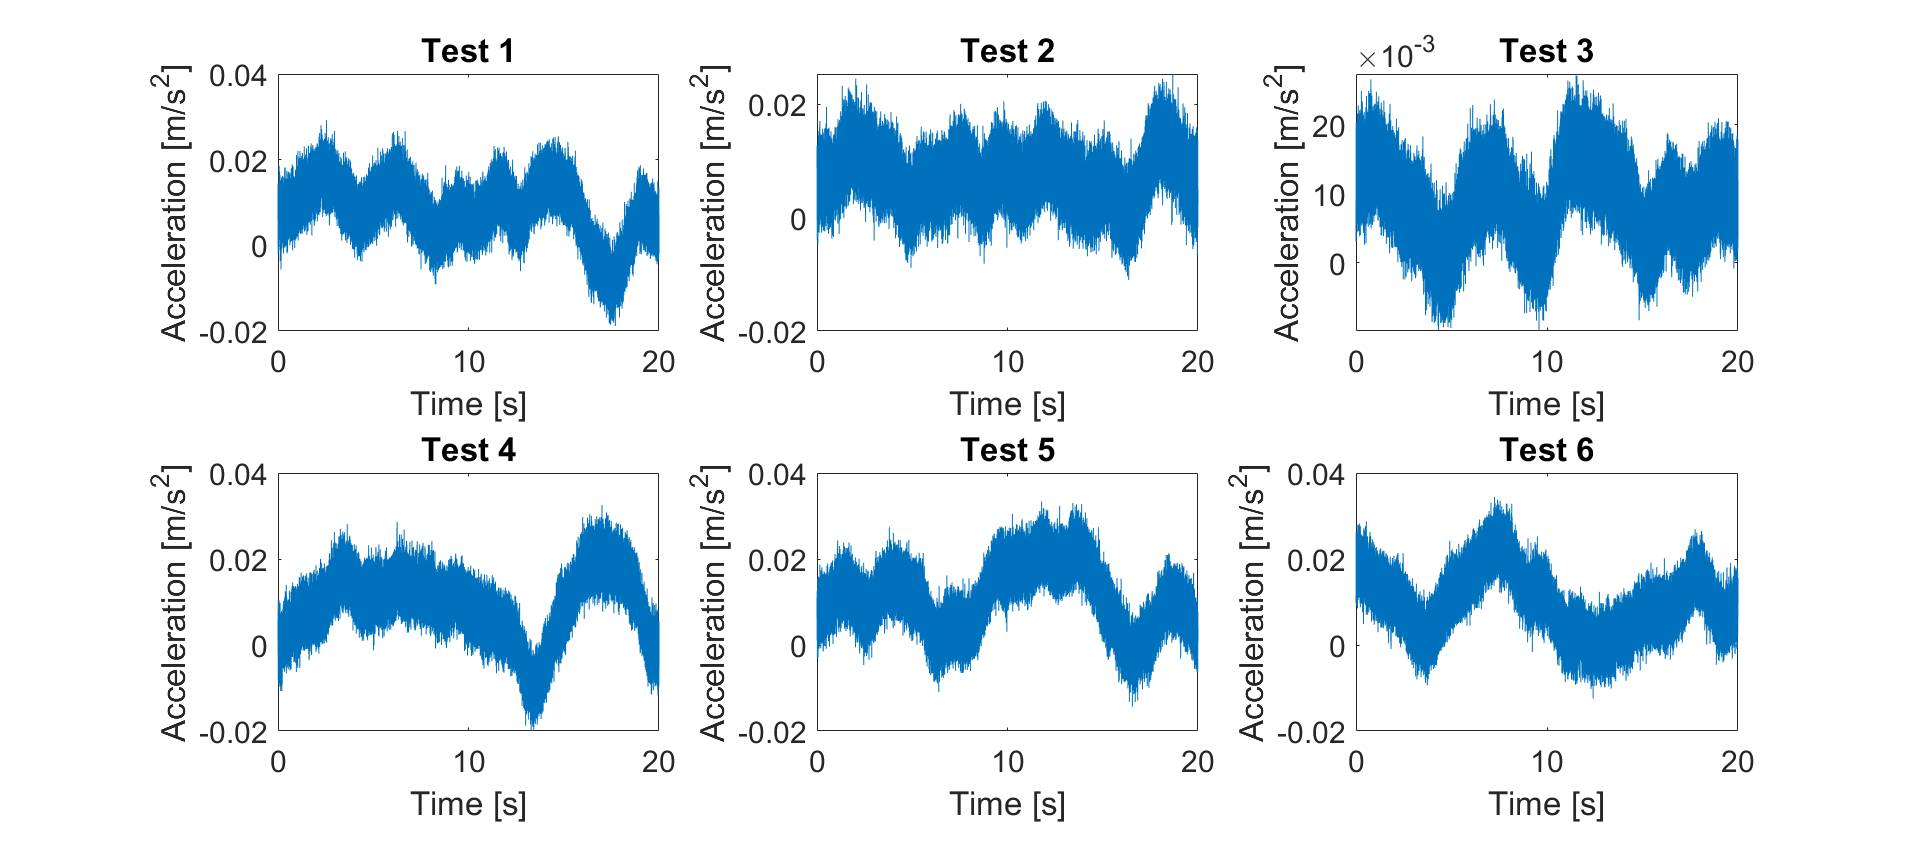
\includegraphics[width=175mm]{images/2_acc1.png}
		\caption{Data from accelerometer 1}
	\end{figure}
	
	\begin{figure}[H]
		\centering
		\includegraphics[width=175mm]{images/2_acc2.png}
		\caption{Data from accelerometer 2}
	\end{figure}

	\begin{figure}[H]
		\centering
		\includegraphics[width=175mm]{images/2_acc3.png}
		\caption{Data from accelerometer 3}
	\end{figure}
	
	These values of noise are quite low. As we will see, they do not affect on the next experiments.
	
	\medskip
	 
	\item In order to find the power spectral density of each curve, I followed the general procedure starting computing FFT (Fast Fourier Transform). I calculated the PSD (Power Spectral Density) non squared because the squared one would have produced a too small signal to be handle by MATLAB. \\
	I also took the mean among the six tests and the standard deviation so that I could plot them together. \\
	
	\begin{figure}[H]
		\centering
		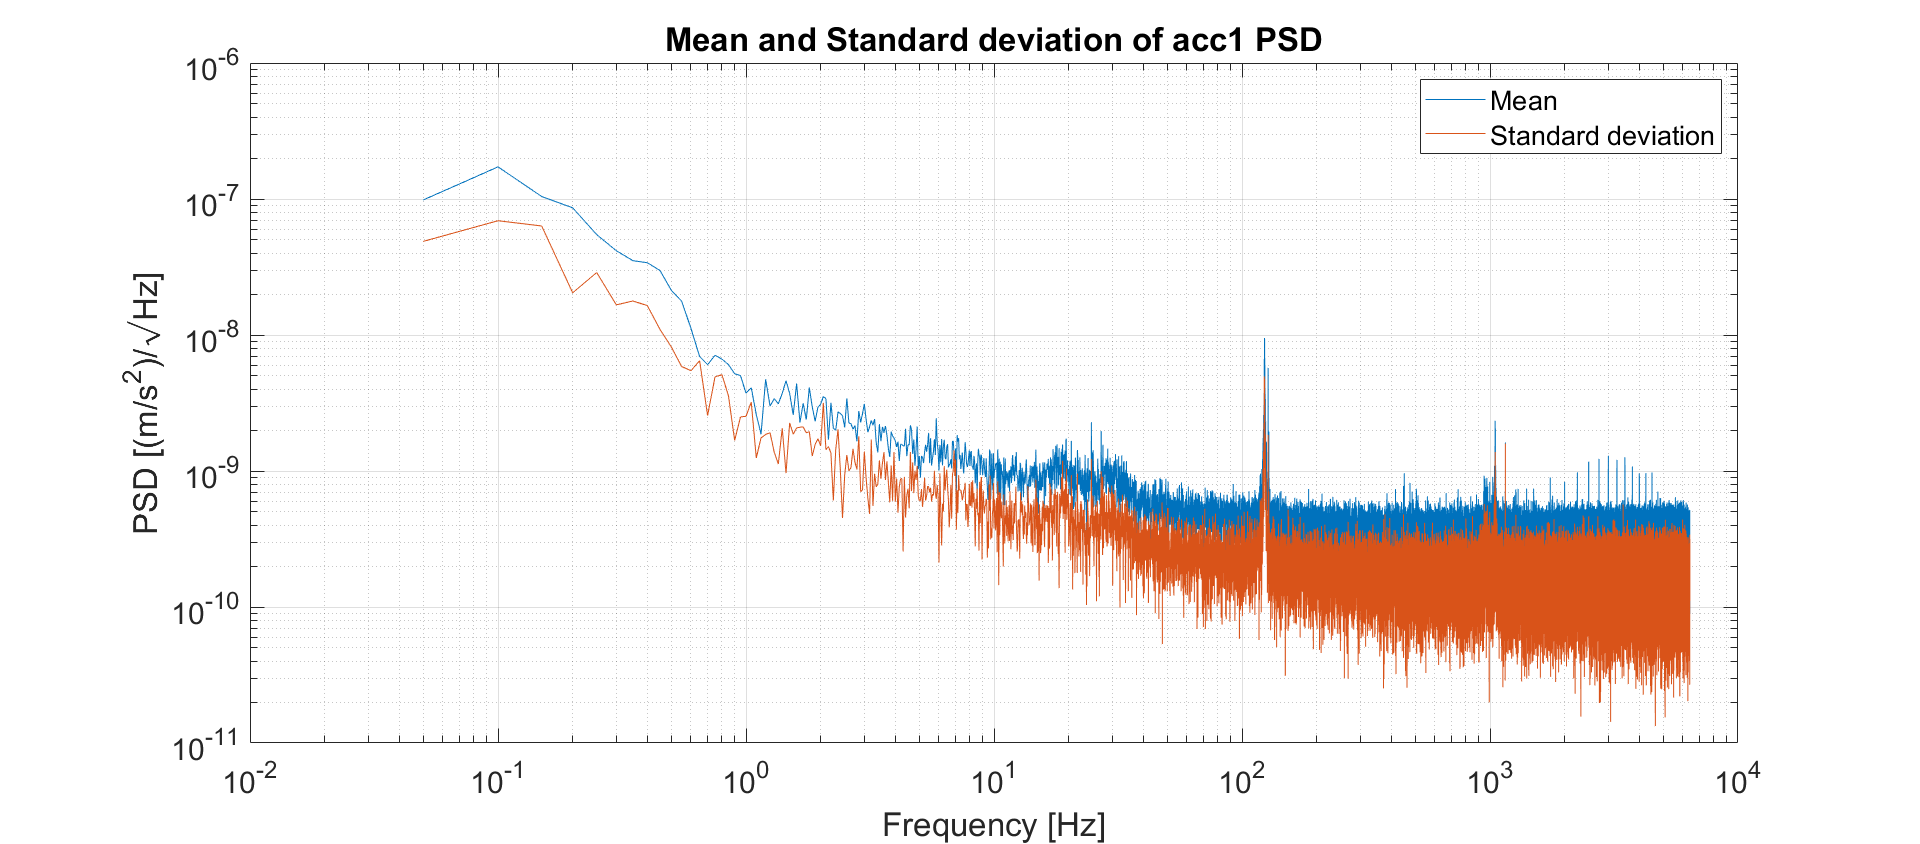
\includegraphics[width=150mm]{images/2_meanstd1.png}
		\caption{PSD of accelerometer 1}
	\end{figure}

	\begin{figure}[H]
		\centering
		\includegraphics[width=150mm]{images/2_meanstd2.png}
		\caption{PSD of accelerometer 2}
	\end{figure}
	
	\begin{figure}[H]
		\centering
		\includegraphics[width=150mm]{images/2_meanstd3.png}
		\caption{PSD of accelerometer 3}
	\end{figure}

	By observing the graphs you can see that there are some peaks along the response. Their locations are closed to the analytical natural frequencies of the pinned-pinned beam. A particularity is that in the signal of the first accelerometer there isn't the peak at the second natural frequency, probably due to the fact that it is located in the node of the related mode shape. This happens also for the other accelerometers for the last three nodes, but with a minor effect. 
	
	
\end{enumerate}	

\newpage
\section{Impact hammer excitation}
After analyzing the beam without input, we studied its behavior following an excitation by a impact hammer. The hitting point is P1, located in the middle of the beam. \\
As previously, force and accelerations have been measured by the instruments. 
    
\begin{enumerate}
	
	\item The model of the hammer is 086C03, and the hardest tip was mounted. By viewing its frequency response, it reaches -3 dB at around 2000 Hz. For this reason the range of interest is\\ $f_{range} =$ {$20\div2230$} Hz.
	\begin{figure}[H]
		\centering
		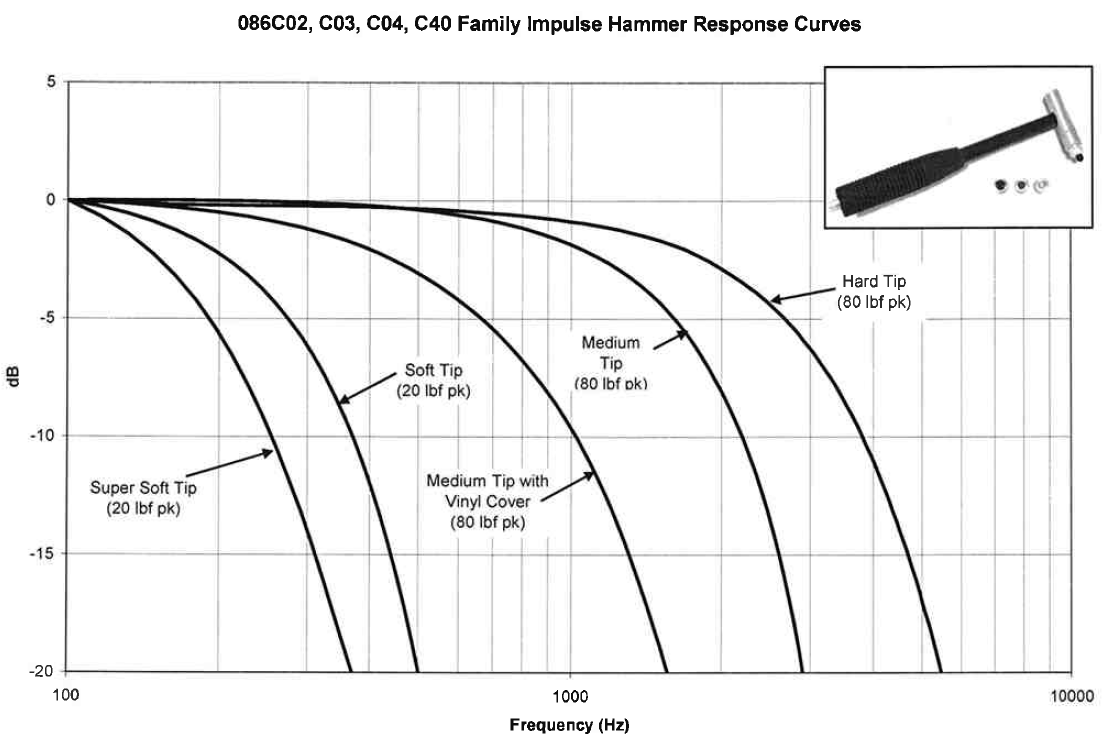
\includegraphics[width=100mm]{images/hammer.png}
		\caption{Hammer response curve for different tips}
	\end{figure}
	
	\medskip
	
	\item The pictures below show the accelerations measured by the three accelerometers in each tests along the time duration.
	
	\begin{figure}[H]
		\centering
		\begin{subfigure}[b]{0.3\textwidth}
			\centering
			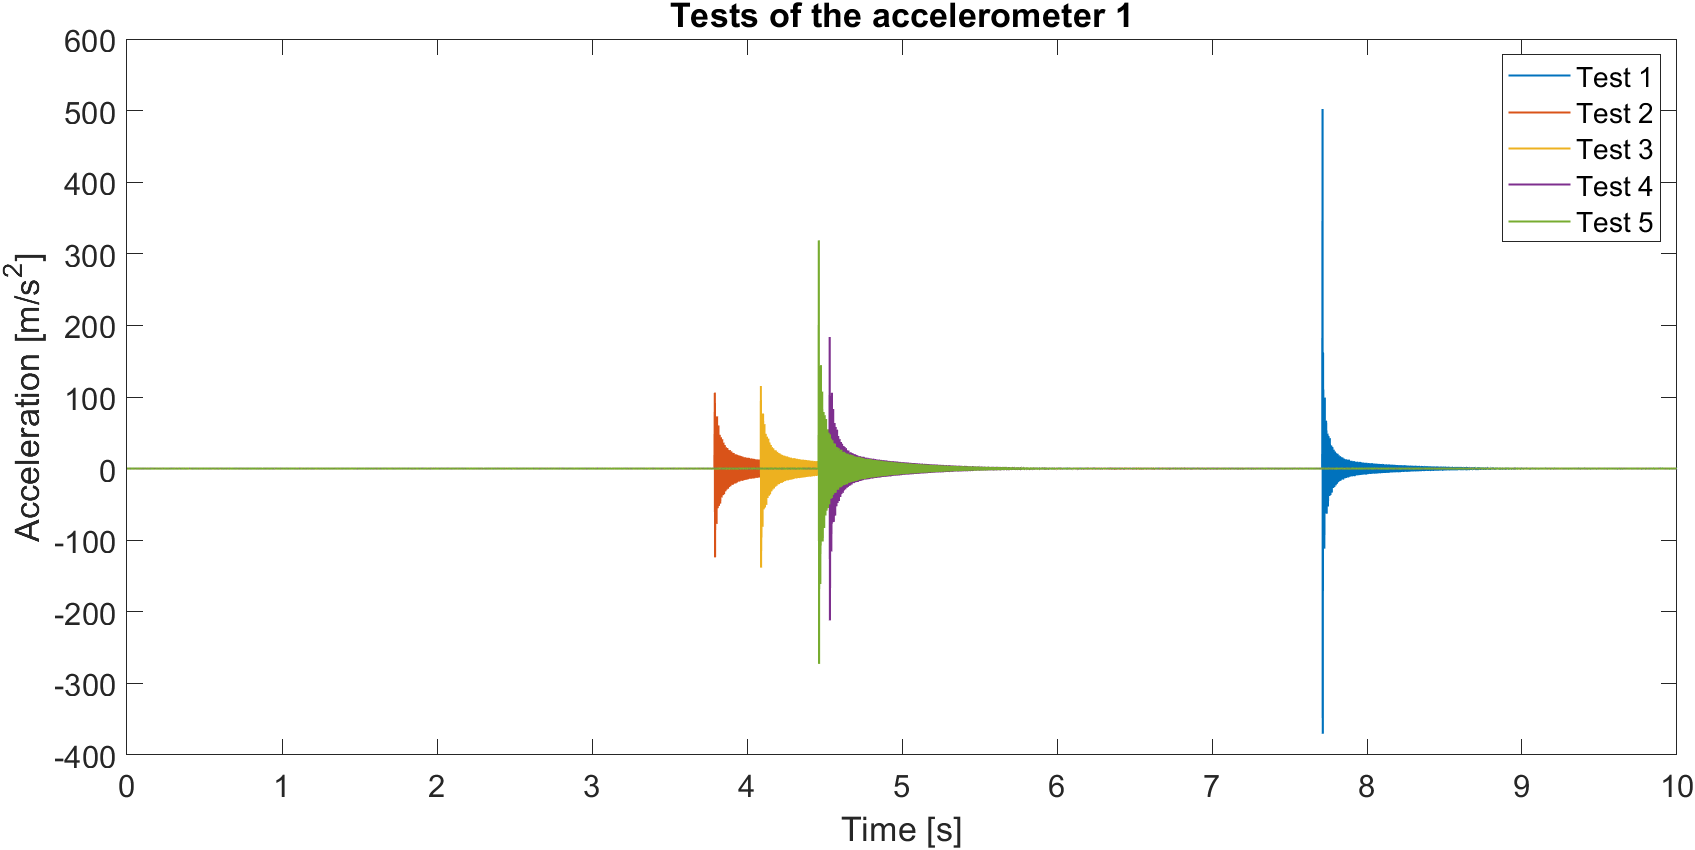
\includegraphics[width=55mm]{images/3_accelerations1.png}
		\end{subfigure}
		\hfill
		\begin{subfigure}[b]{0.3\textwidth}
			\centering
			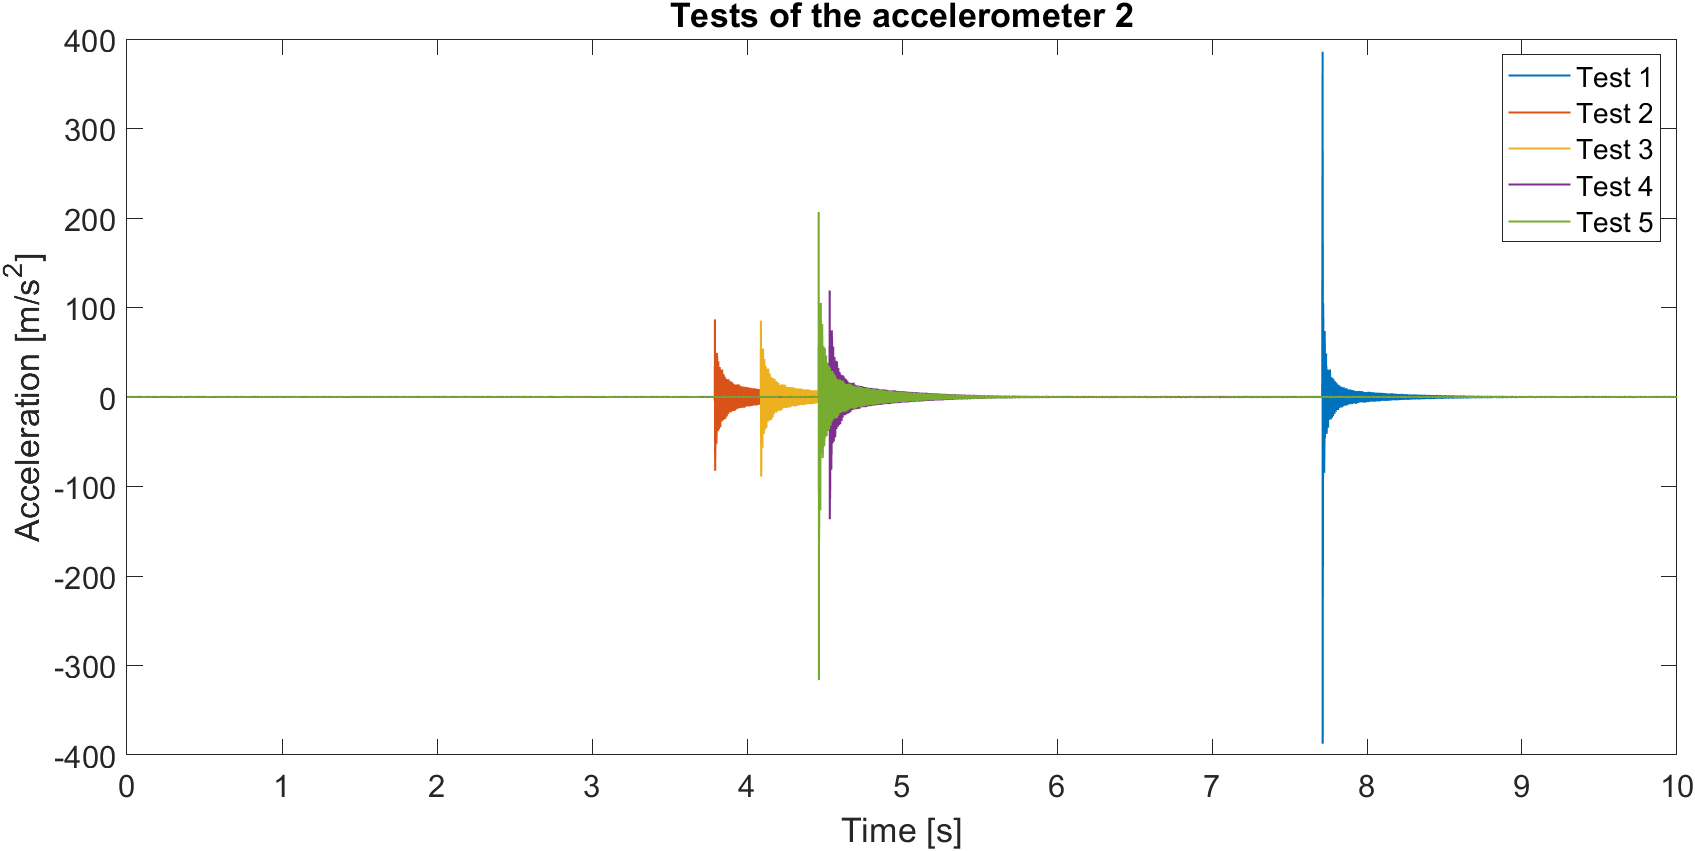
\includegraphics[width=55mm]{images/3_accelerations2.png}
		\end{subfigure}
		\hfill
		\begin{subfigure}[b]{0.3\textwidth}
			\centering
			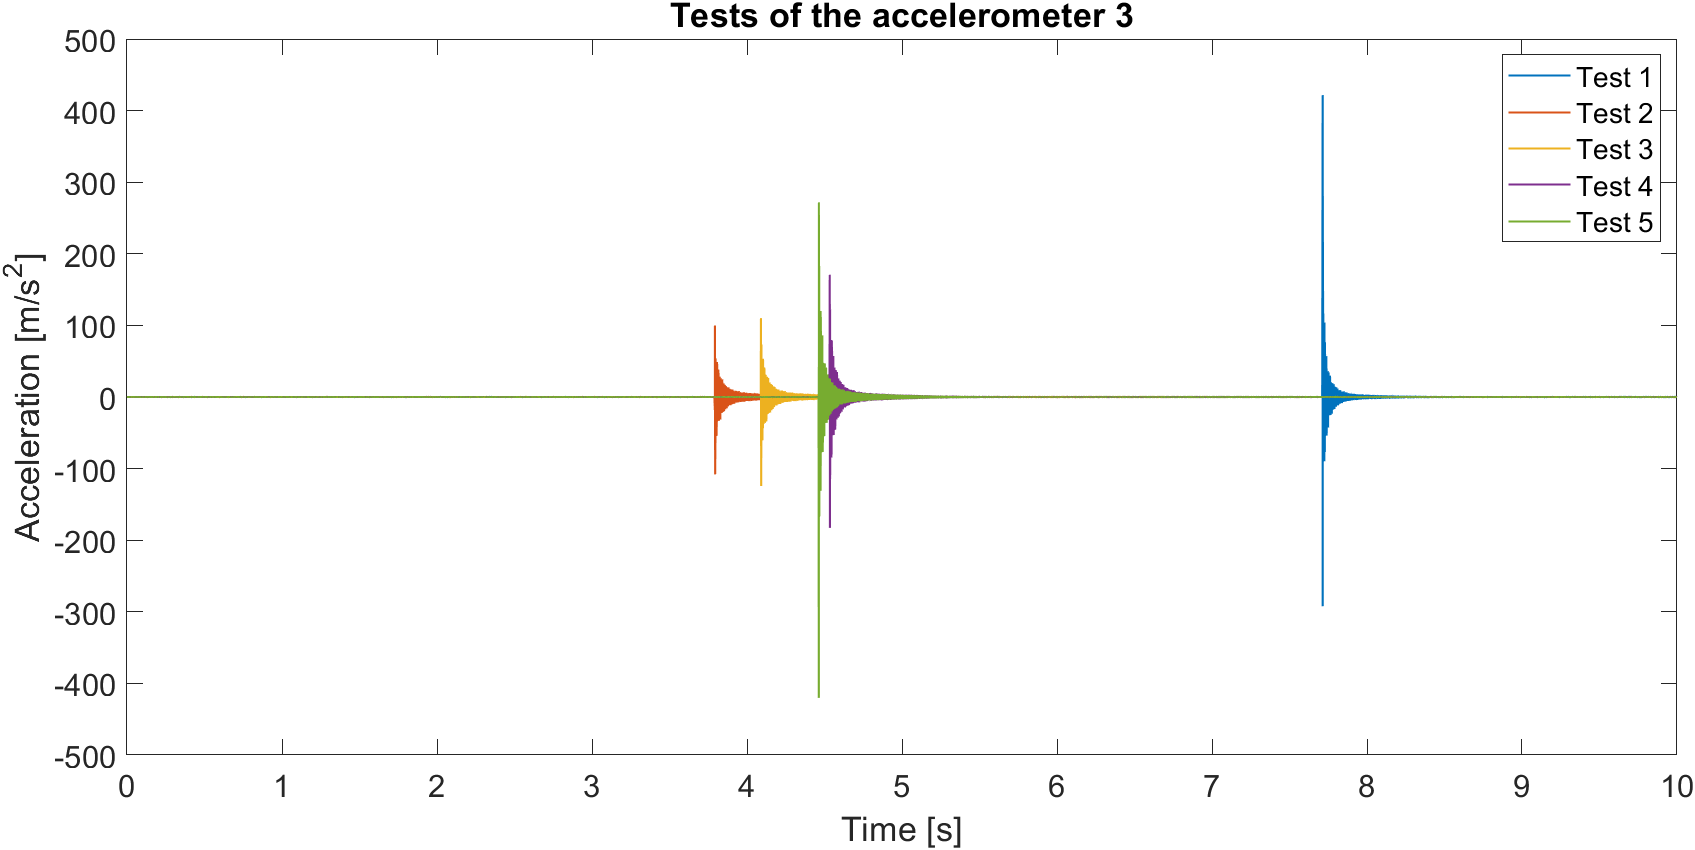
\includegraphics[width=55mm]{images/3_accelerations3.png}
		\end{subfigure}
		\caption{Accelerations measured in all tests}
	\end{figure}
	
	
	In the first test one accelerometer measures an acceleration of around $500\,m/s^2$. Since the maximum measurable acceleration is $\pm 490\,m/s^2$, this test must be discarded.
	Here below I show the difference between this test and a valid one (for example the last).  
	
	\begin{figure}[H]
		\centering
		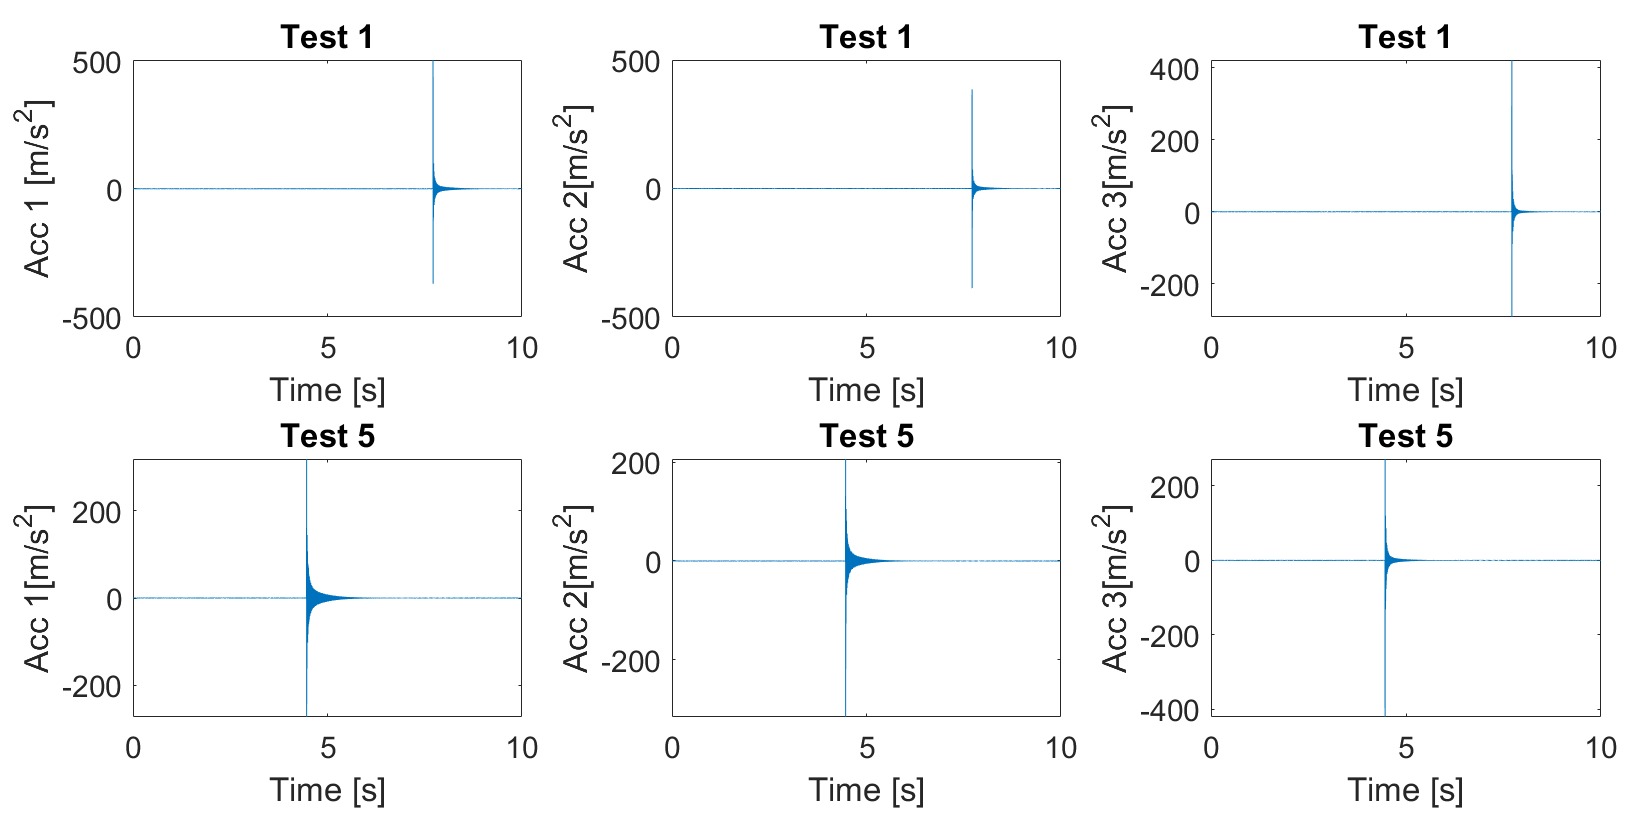
\includegraphics[width=150mm]{images/3_comparison1e5.png}
		\caption{Comparison between the first and the last test}
	\end{figure}

	\medskip
	
	\item From now on, only the valid test will be considered. \\
	I computed the experimental transfer function with the MATLAB function \texttt{tfestimate} specifying the input (force) and the output (acceleration).
	I took the module (with \texttt{abs}) to plot the results. 
	 \begin{figure}[H]
	 	\centering
	 	\includegraphics[width=150mm]{images/3_tfacc1.png}
	 	\caption{Transfer functions accelerometer 1}
	 \end{figure}
	\begin{figure}[H]
		\centering
		\includegraphics[width=150mm]{images/3_tfacc2.png}
		\caption{Transfer functions accelerometer 2}
	\end{figure}
	\begin{figure}[H]
		\centering
		\includegraphics[width=150mm]{images/3_tfacc3.png}
		\caption{Transfer functions accelerometer 3}
	\end{figure}

	\medskip

	\item In the next pictures I compare the analytical TFs (taken by Maple) with the experimental ones.
	\begin{figure}[H]
		\begin{subfigure}[b]{0.5\textwidth}
			\centering
			\includegraphics[width=75mm]{images/1_tf1_1.png}
		\end{subfigure}
		\hfill
		\begin{subfigure}[b]{0.5\textwidth}
			\centering
			\includegraphics[width=75mm]{images/3_meanstd1.png}
		\end{subfigure}
		\caption{Analytical TF and Experimental TF accelerometer 1 (hammer)}
	\end{figure}
	
	\begin{figure}[H]
		\begin{subfigure}[b]{0.5\textwidth}
			\centering
			\includegraphics[width=75mm]{images/1_tf1_2.png}
		\end{subfigure}
		\hfill
		\begin{subfigure}[b]{0.5\textwidth}
			\centering
			\includegraphics[width=75mm]{images/3_meanstd2.png}
		\end{subfigure}
		\caption{Analytical TF and Experimental TF accelerometer 2 (hammer)}
	\end{figure}
	
	\begin{figure}[H]
		\begin{subfigure}[b]{0.5\textwidth}
			\centering
			\includegraphics[width=75mm]{images/1_tf1_3.png}
		\end{subfigure}
		\hfill
		\begin{subfigure}[b]{0.5\textwidth}
			\centering
			\includegraphics[width=75mm]{images/3_meanstd3.png}
		\end{subfigure}
		\caption{Analytical TF and Experimental TF accelerometer 3 (hammer)}
	\end{figure}

	As a first consideration, we can say that the graphs are very similar (with the experimental one less accurate, obviously). The peaks are positioned in proximity of the natural frequencies of the pinned-pinned beam.
	We can do the comparison with the fixed-fixed beam study: since in a real experiment it's very difficult to recreate an ideal pinned-pinned beam, and so some effects appear in any case: small peaks are visible closed to the natural frequencies of the fixed-fixed beam.
\end{enumerate}	



\newpage
\section{Shaker excitation}
In this other experiment, the beam is excited with an electro dynamic shaker. The point of application is $P_4$, at a distance of $L/8$ from the left pin. \\
The force is generated as a variable-frequency signal and the excitation has been subdivided in 7 frequency ranges (that cover the overall range of interest $20\div2230$ Hz). Each input is repeated 4 times.

\begin{table}[h]
	\centering
	\begin{tabular}{c c c c c c} 
		\toprule
		Range number & $f_{min}$ (Hz) & $f_{max}$ (Hz) & Duration (s) & Sampl. freq. (Hz) & Repetitions \\ 
		\midrule	    		   	    		
		1 & 20 	 & 430 	& 20 & 12800 & 4 \\	
		2 & 400  & 730 	& 20 & 12800 & 4 \\
		3 & 700  & 1030 & 20 & 12800 & 4 \\
		4 & 1000 & 1330 & 20 & 12800 & 4 \\
		5 & 1300 & 1630 & 20 & 12800 & 4 \\
		6 & 1600 & 1930 & 20 & 12800 & 4 \\
		7 & 1900 & 2230 & 20 & 12800 & 4 \\
		\bottomrule
	\end{tabular}
	\caption{Frequency ranges used to excite the beam with the shaker}
\end{table}  
\begin{enumerate}
	\item Since we have one more variable, we'll have a 4-dimensional matrix of data (just  more computationally expensive). The procedure is similar to the previous part but it's necessary to do a for loop more. \\
	I computed the estimate transfer function for each accelerometers, then the mean among four repetition, and the corresponding standard deviation.
	
	\medskip
	
	\item In order to do a single plot, I had to merge the 7 frequency ranges. We can see below the comparison of the result with the analytical TFs.

	\begin{figure}[H]
		\begin{subfigure}[b]{0.5\textwidth}
			\centering
			\includegraphics[width=75mm]{images/1_tf2_1.png}
		\end{subfigure}
		\hfill
		\begin{subfigure}[b]{0.5\textwidth}
			\centering
			\includegraphics[width=75mm]{images/4_meanstd1.png}
		\end{subfigure}
		\caption{Analytical TF and Experimental TF accelerometer 1 (shaker)}
	\end{figure}
	
	\begin{figure}[H]
		\begin{subfigure}[b]{0.5\textwidth}
			\centering
			\includegraphics[width=75mm]{images/1_tf2_2.png}
		\end{subfigure}
		\hfill
		\begin{subfigure}[b]{0.5\textwidth}
			\centering
			\includegraphics[width=75mm]{images/4_meanstd2.png}
		\end{subfigure}
		\caption{Analytical TF and Experimental TF accelerometer 2 (shaker)}
	\end{figure}
	
	\begin{figure}[H]
		\begin{subfigure}[b]{0.5\textwidth}
			\centering
			\includegraphics[width=75mm]{images/1_tf2_3.png}
		\end{subfigure}
		\hfill
		\begin{subfigure}[b]{0.5\textwidth}
			\centering
			\includegraphics[width=75mm]{images/4_meanstd3.png}
		\end{subfigure}
		\caption{Analytical TF and Experimental TF accelerometer 3 (shaker)}
	\end{figure}
	Also in this case the plots are similar and the peaks are in the correct position, closed to the natural frequencies of the pinned-pinned beam.
\end{enumerate}	

\footnotesize
\newpage
\hypersetup{linkcolor = black}
\listoffigures
\listoftables
\end{document}
